%%
%% Author: samuelblattner
%% 2019-01-20
%%

% Preamble
\documentclass{ffhsthesis}

% Packages
\usepackage{amsmath}
\usepackage[utf8]{inputenc}
\usepackage[bibstyle=apa,backend=biber]{biblatex}

% Listings
\usepackage{listings}
\usepackage{color}
\usepackage{tabularx}

\definecolor{codegreen}{rgb}{0,0.6,0}
\definecolor{codegray}{rgb}{0.5,0.5,0.5}
\definecolor{codepurple}{rgb}{0.58,0,0.82}
\definecolor{backcolour}{rgb}{0.95,0.95,0.92}

\lstdefinestyle{mystyle}{
backgroundcolor=\color{backcolour},
commentstyle=\color{codegreen},
keywordstyle=\color{magenta},
numberstyle=\tiny\color{codegray},
stringstyle=\color{codepurple},
basicstyle=\footnotesize,
breakatwhitespace=false,
breaklines=true,
captionpos=b,
keepspaces=true,
numbers=left,
numbersep=5pt,
showspaces=false,
showstringspaces=false,
showtabs=false,
tabsize=2
}

\lstset{style=mystyle}
\addbibresource{sema-samuel-blattner.bib}
\usepackage[hidelinks]{hyperref}
\usepackage{glossaries}

\makeglossaries

\newglossaryentry{neuron}
{
name=Neuron,
plural=Neuronen,
description="Ein Neuron ist ein…"
}

\newglossaryentry{Tokenizer}
{
name=Tokenizer,
plural=Tokenizers,
description="Ein Tokenizer ist ein..."
}
\makeglossaries
\makeglossary

% Document
\begin{document}

    \dokumentTyp{Seminararbeit}
    \studiengang{INF/WI}
    \title{Recurrent Neuronal Networks als Kreativitätswerkzeug für Gastronomiebetriebe}
    \titelbild[height=5cm,width=10cm]{ffhslogo}  % optional
    \author{Samuel Blattner}
    \wohnort{Zürich}

    \referentin{Dr. Heinrich Zimmermann\\ BSc INF 2015, ZH5-Mo, FS19}
    \eingereichtBei{Dr. Heinrich Zimmermann\\ BSc INF 2015, ZH5-Mo, FS19}

    \maketitle

    \begin{zusammenfassung}
        In dieser Arbeit untersucht, ob Rekurrente Neuronale Netze (RNNs) dazu verwendet werden können,
        epochenabhängige, neue Bezeichnungen von Gerichten als Kreativitätswerkzeug für die Gastronomie zu erzeugen.
        Dazu wird ein RNN in verschiedenen Konfigurationen mit dem Datensatz «What's on the Menu» trainiert und
        die Ausgaben systematisch analysiert und auf ihre Tauglichkeit überprüft.
        Die Arbeit kommt zum Schluss, dass das Modell durchaus fähig ist, neue und lesbare Bezeichnungen zu erzeugen,
        dass jedoch die Vielfallt zu begrenzt ist.
    \end{zusammenfassung}

    \begin{abstract}
        This work investigates if Recurrent Neuronal Networks (RNNs) can be utilized to generate new names for
        dishes based on epochs.
        For this purpose, an RNN is trained on the «What's on the menu» dataset and is systematically analyzed and
        tested for its usefulness.
        This work concludes that a model can very well be used to generate new and readable names for dishes, but
        that the variety is limited.
    \end{abstract}

    \setcounter{tocdepth}{1}
    \tableofcontents

    \startThesis % Befehl muss vor dem ersten chapter stehen (Seitennummerierung!)

    \chapter{Einleitung}
\label{ch:introduction}

Die Gastronomie hat sich im vergangenen Jahrzehnt nach eigener Wahrnehmung des Autors zu einem äusserst populären Thema entwickelt.
Haupttreiber dafür sind sicherlich Social Media, auf denen kreative Lokale, ausgefallene Gerichte und besondere Momente weltweit geteilt werden.
Andererseits tragen auch ein neues Ernährungsbewusstsein, die weltweite Mobilität sowie Berichterstattungen über Gastronomiebetriebe, beispielsweise als TV-Serie, zum wachsenden Interesse bei.
Der Markt ist hart umkämpft, und Restaurants kommen und gehen insbesondere in Stadtgebieten in hohen Raten, wie eine neuere Statistik der Stadt Zürich zeigt\footnote{https://www.zkb.ch/media/pub/coporate/zuerich-in-zahlen/kt-zh-zahlen-223653.pdf}.
Der gesättigte Markt zwingt die Betriebe zu Effizienz, Innovation und zu möglichst hoher Qualität.
Unlängst hat deshalb auch die Digitalisierung in Gastronomiebetrieben Einzug gehalten, werden doch zumindest Reservationen immer häufiger online getätigt\footnote{https://www.lunchgate.info/blog/gastronomie-digitalisierung}, Bestellungen via Tablet
direkt in die Küche gesendet und Rechnungen per App unter Freunden aufgeteilt.
All diese Entwicklungen beschäftigen sich primär mit der Automatisierung von Prozessen.
Wie aber können Gastronomiebetriebe in anderen Bereichen, wie z.B. der Kreativität unterstützt werden?
Diese Arbeit geht folgender Frage nach: «Kann ein neuronales Netz durch Training mit einfachen Namen von Gerichten sinnvolle, neue und parameterabhängige Namen erzeugen?»
Diese Arbeit untersucht, ob und wie ein Neuronales Netz als Kreativitätswerkzeug bzw. Namensgenerator für Speisen verwendet werden kann.

    \chapter{Modell}
\label{ch:model}

Dieser Teil beschreibt das der Arbeit zugrunde liegende Modell.
Das Modell wird hierbei in seiner finalen Ausführung dargestellt.
Dieser liegen diverse Iterationen von Experimenten und Verbesserungen zugrunde, die jedoch für das Verständnis des
Modells keine Relevanz haben und auf die nicht weiter eingegangen wird.
Einzig die Behebung eines Implementierungsfehlers sowie die damit verbundene Änderung in der Art und Weise, wie das Modell trainiert wird,
sollen kurz beleuchtet werden, da sie für den Leser wertvolle Hinweise für eigene Implementierungen bieten können.

\section{Daten \& Training}
\label{sec:model-data-training}

In diesem Abschnitt werden die Trainingsdaten für das Modell analysiert und beschrieben.
Als Lerngrundlage für den Algorithmus dienen rund 400000 Namen von Gerichten.
Diese sind im Kaggle-Datensatz «What's on the menu»\footnote{https://www.kaggle.com/nypl/whats-on-the-menu}\footnote{http://nypl.github.io/menus-api/} enthalten.
Der Unterdatensatz «Dish.csv» enthält folgende Struktur:


\begin{center}
    \resizebox{\textwidth}{!}{
    \begin{tabular}{ |r|l|r|r|r|r|r|r| }
        \hline
        \textbf{id} & \textbf{name} & \textbf{menus\_appeared} & \textbf{times\_appeared} & \textbf{first\_appeared} & \textbf{last\_appeared} & \textbf{lowest\_price} & \textbf{highest\_price} \\
        \hline
        1 & Consomme printaniere royal  &    8 &    9 & 1897 & 1927 & 0.2  & 0.4 \\
        \hline
        2 & Chicken gumbo               &  110 &  116 & 1895 & 1960 & 0.1  & 0.8 \\
        \hline
        3 & Tomato aux croutons         &   13 &   13 & 1893 & 1917 & 0.25 & 0.4 \\
        \hline
        4 & Onion au gratin             &   41 &   41 & 1900 & 1971 & 0.25 & 1   \\
        \hline
        5 & Radishes                    & 3265 & 3349 & 1854 & 2928 & 0    & 25  \\
        \hline
        6 & Chicken soup with rice      &   48 &   49 & 1897 & 1961 & 0.1  & 0.6 \\
        \hline
        … & … & … & … & … & … & … & … \\
        \hline
    \end{tabular}
    }
\end{center}

Für die Arbeit relevant ist vorerst lediglich die \textit{name}-Spalte.
Sie enthält Bezeichungen von Gerichten in mehreren Sprachen.

Für das Training eines ersten Modells wird folgende Spezifikation verwendet:

Batches: 100
Batchsize: 50
Epochen: 50
RNN-Units: 64
RNN-Layers: 1
Textlänge: 15

Für die Validierung pro Epoche werden jeweils die weiteren Zeilen, die auf das Trainingsset folgen, verwendet.



\section{Formale Definition}
\label{sec:model-definition}

Weil sie fähig sind, zeitliche Zustände zu speichern, eignen sich Rekurrente Neuronale Netze (in der restlichen Arbeit wird die Abkürzung «RNN» verwendet) besonders gut, um Sequenzen zu lernen.
Die natürliche Sprache ist eine Sequenz von Wörtern, die in sich wiederum aus einer Sequenz von Buchstaben bestehen.
Deshalb kommen RNNs bis heute in vielen Gebieten von natürlichsprachlicher Textverarbeitung zum Einsatz.

Die Besonderheit eines RNN's liegt darin, dass – anders als bei einfachen neuronalen Netzen – die \glspl{neuron} nicht nur den Wert der vorangehenden Netzschicht als
Eingangswert erhalten, sondern auch den Ausgangswert des vorangehenden Zeitschritts ihrer selbst.
Jedes \gls{neuron} speichert den Zustand der bisherigen Zeitschritte als sog. «hidden state», der mit der Variable $ h $ gekennzeichnet wird (siehe Abb. \ref{fig:rnn-model-definition}).
Für nähere Details zur Architektur und Funktionsweise sei auf die exzellente Beschreibung in \autocite{geron} verwiesen.

\begin{figure}
    \centering
    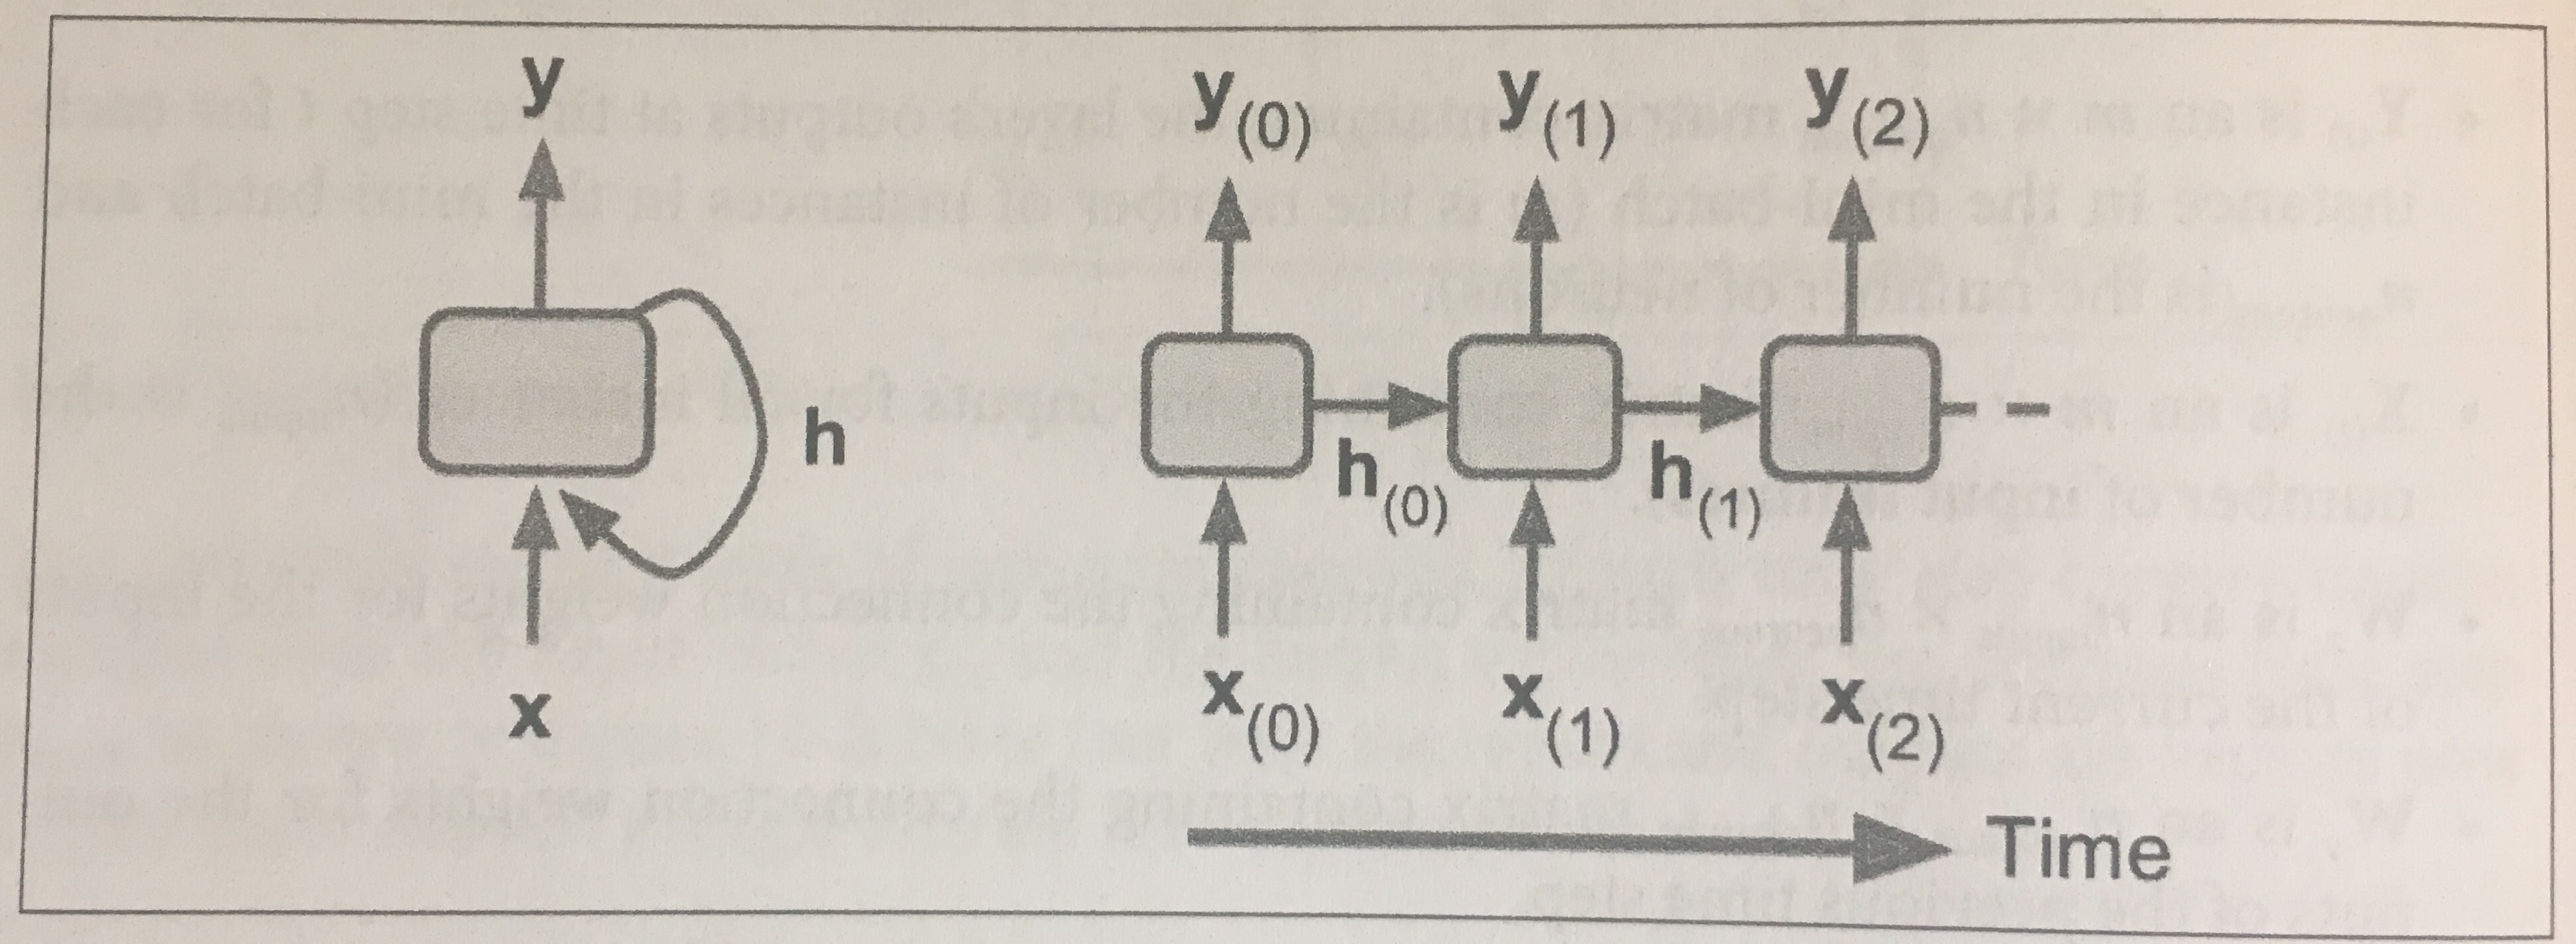
\includegraphics[width=0.75\linewidth]{images/model/model-rnn-definition.jpg}
    \caption[RNN Modell]{RNN Modell \autocite{geron}}
    \label{fig:rnn-model-definition}
\end{figure}

Zwei gut bekannte Probleme, die einfache RNN-Memory-Zellen aufweisen sind einerseits das sog. «Exploding/Vanishing Gradient Problem», bei dem insbesondere in mehrschichtigen neuronalen Netzen
die propagierten Werte «explodieren» oder gegen null «verschwinden», andererseits das Problem, dass anfangs eingespeiste Informationen gegen Ende der Sequenz verloren gehen \autocite{geron}.
Zur Lösung dieser Problem wurden sog. «Long-Short-Term Memory Cells» (LSTM)\autocite{lstm} und später sog. «Gated Recurrent Units» (GRU)\autocite{gru} entwickelt.
Weil sich beide «Gedächtniszellen» als sehr erfolgreich bewiesen haben, werden einfache RNN-Zellen schon fast nicht mehr verwendet.


\section{Implementierung}
\label{sec:model-implementation}

Für den Aufbau und das Training werden TensorFlow 2.0\footnote{https://www.tensorflow.org/beta} sowie das mittlerweile darin integrierte Framework Keras\footnote{https://keras.io/} verwendet.
Der Code ist auf Github\footnote{https://github.com/samuelblattner/ffhs-sema} frei verfügbar.
Die Implementierung kann grundsätzlich in drei Komponenten aufteilt werden:

\paragraph{Builder (build.py)} Die Builder-Komponente übernimmt die Aufgabe, das RNN-Modell mit Keras nach bestimmten Vorgaben aufzubauen (z.B. Anzahl LSTM-Einheiten, Anzahl Schichten, …).
Weil Neuronale Netze auf arithmetischen Operationen beruhen, müssen die Eingabezeichen in Zahlen umgewandelt werden.
Diese Aufgabe übernimmt ein sog. «\glq{Tokenizer}».
Die Komponente gibt als Rückgabewert einersets das kompilierte Modell sowie andererseits einen Tokenizer zurück, der numerische Repräsentationen für sämtliche im Datensatz enthaltenen Zeichen (=Vokabular) enthält.

\paragraph{Loader} Der Loader übernimmt die Aufgabe, die Trainings- wie auch Validierungsdaten bereitszustellen.
Das Training des Modells wird im sog. Mini-Batch-Verfahren vollführt.
Der Loader lädt damit mit einem Python-Generator für jede Trainingsepoche nacheinander mehrere Ausschnitte des Gesamtdatensatzes (siehe Listing \ref{lst:mini-batch-loader}, Zeile 3).
Dies ermöglicht, beliebig grosse Datensätze zu bearbeiten, da immer nur der Speicherbedarf eines Mini-Batches benötigt wird.
Der Loader implementiert zudem ein Offset (Zeile 13), mit dem der Datensatz «vorgespult» werden kann.
Damit ist es möglich, vom gleichen Datensatz sowohl das Trainingsset wie auch das Validierungsset zu entnehmen.
Statt vom Anfang des Datensatzes, startet das Validierungsset jedoch viel weiter hinten im Datensatz, im Idealfall – und bei genügend grossem Datensatz – ausserhalb des Bereichs, den das Trainingsset jemals erreichen wird.

\begin{lstlisting}[language=Python, caption=Mini-Batch Loader, label=lst:mini-batch-loader]
    ...
    # Load mini-batch
    for dataframe in read_csv(
        filepath_or_buffer='data.csv',
        delimiter=',',
        header=0,
        chunksize=1000):

        # Iterate over lines in mini-batch
        for row in dataframe[dataframe.columns[1]]:
            ...

            if self.__offset > 0 and offset_lines_skipped < self.__offset:
                offset_lines_skipped += 1
                continue
                ...
\end{lstlisting}

Der Loader übernimmt zudem die Aufgabe, die Textsequenzen in einzelne Trainingseinheiten zu zerlegen.
Eine Trainingseinheit besteht immer aus einer konstanten Anzahl Zeichen (Fenstergrösse) und einem Zielzeichen.
Zudem wird am Schluss eine Stoppmarke («<end>») angefügt, die dem Modell das Ende der Sequenz signalisiert.
Ist eine Trainingssequenz kürzer als die Fenstergrösse, wird sie mit Platzhalter Zeichen aufgefüllt («padding»).
Ist eine Trainingssequenz länger als die Fenstergrösse, so wird sie abgeschnitten.
und Zeichen um Zeichen in mehreren Trainingsschritten durch das Fenster geschoben (siehe Tabelle \ref{tab:splitting-into-training-units}).
Der letzte Buchstabe wird jeweils als Zielwert abgeschnitten und in einem separaten Array zurückgeliefert (y-Wert).
Gleichzeitig werden die Buchstabensequenzen mit dem zuvor erwähnten Tokenizer in Vokabular-Indizes umgewandelt.
Da die Ausgabe des Modells eine Wahrscheinlichkeitsverteilung für alle Buchstaben in Form eines Vektors sein wird (Wertebereich 0.0 - 1.0), ist es
für ein optimales Training erforderlich, auch die Eingabe ins Modell entsprechend umzuformen.
Die Vokabular-Indizes werden umgewandelt in sog. «One-Hot-Vektoren».
Ein One-Hot-Vektor besteht aus sovielen Komponenten, wie das Vokabular Zeichen enthält.
Die Komponenten mit dem Index des entsprechenden Zeichens wird auf $ 1.0 $ gesetzt, alle anderen Komponenten bleiben $ 0.0 $.
Der Eingabevektor ist somit gewissermassen ebenfalls eine Wahrscheinlichkeitsverteilung, allerdings hat genau ein Zeichen die Wahrscheinlichkeit $ 100\% $ (das nächste Zeichen in der Sequenz), während
alle anderen Zeichen die Wahrscheinlichkeit $0.0\%$ haben.
Hat das nächste Zeichen «B», das ins Modell eingegeben werden soll, den Tokenizer-Index 2 (bei einer Vokabulargrösse von insgesamt 5 Zeichen), so würde daraus der One-Hot-Vektor $ (0.0, 0.0, 1.0, 0.0, 0.0, 0.0)^{T} $ gebildet.
Listing \ref{lst:one-hot-encoding} zeigt, wie die Konvertierungsschritte von Zeichen bis One-Hot-Vektor mit den von Keras bereitsgestellten Utility-Funktionen einfach erledigt werden können.

\begin{table}
    \centering
    \footnotesize
    \begin{tabularx}{0.75\textwidth}{|>{\hsize=.1\hsize}X|>{\hsize=.1\hsize}X|>{\hsize=.1\hsize}X|>{\hsize=.1\hsize}X|>{\hsize=.1\hsize}X|>{\hsize=.1\hsize}X|>{\hsize=.1\hsize}X|>{\hsize=.1\hsize}X|>{\hsize=.1\hsize}X||>{\hsize=.1\hsize}X|}
    \hline
    \textbf{0} & \textbf{1} & \textbf{2} & \textbf{3} & \textbf{4} & \textbf{5} & \textbf{6} & \textbf{7} & \textbf{8} & \textbf{Ziel} \\\hline
            pad & pad & pad & pad & pad & pad & pad & pad & pad & C \\\hline
            pad & pad & pad & pad & pad & pad & pad & pad & C & h \\\hline
            pad & pad & pad & pad & pad & pad & pad & C & h & i \\\hline
            pad & pad & pad & pad & pad & pad & C & h & i & c \\\hline
            pad & pad & pad & pad & pad & C & h & C & c & k \\\hline
            pad & pad & pad & pad & C & h & i & c & k & e \\\hline
            pad & pad & pad & C & h & i & c & k & e & n \\\hline
            pad & pad & C & h & i & c & k & e & n & ' ' \\\hline
            pad & C & h & i & c & k & e & n & ' ' & C \\\hline
            C & h & i & c & k & e & n & ' ' & C & u \\\hline
            h & i & c & k & e & n & ' ' & C & u & r \\\hline
            i & c & k & e & n & ' ' & C & u & r & r \\\hline
            c & k & e & n & ' ' & C & u & r & r & y \\\hline
            k & e & n & ' ' & C & u & r & r & y & <end> \\\hline

    \end{tabularx}
    \caption{Zerlegung in Trainingseinheiten am Beispiel der Fenstergrösse 9 (Stellen 0 - 8).
    Der Begriff «Chicken Curry» wird Zeichen um Zeichen durch das Fenster hindurchgeschoben.
    Jede Zeile entspricht einer Trainingseinheit.
    Das Modell versucht das Zielzeichen in der Spalte «Ziel» anhand der Sequenz in den Stellen 0 bis 8 vorherzusagen.}
    \label{tab:splitting-into-training-units}

\end{table}

\begin{lstlisting}[language=Python, caption=Encodierung von Zeichen bis One-Hot-Vektor, label=lst:one-hot-encoding]
    ...

    # Tokenize sequence characters (e.g. ['pad', 'pad', 'B', 'e', 'e', 'r'] -> [2, 2, 5, 4, 4, 1])
    tokenized_char_phrases_X, tokenized_chars_y = windowed_tokenized_sequences[:, :-1], windowed_tokenized_sequences[:, -1]

    # Convert to 1-hot-vector for input into model
    # (e.g. [2, 2, 5, 4, 4, 1] -> [
    #    [0, 0, 1, 0, 0, 0],
    #    [0, 0, 1, 0, 0, 0],
    #    [0, 0, 0, 0, 0, 1],
    #    [0, 0, 0, 0, 1, 0],
    #    [0, 0, 0, 0, 1, 0],
    #    [0, 1, 0, 0, 0, 0],
    # ])
    one_hot_phrases = to_categorical(padded_phrases_X, num_classes=len(tokenizer.index_word) + 1)
    one_hot_ys = to_categorical(tokenized_chars_y, num_classes=len(tokenizer.index_word) + 1)
    ...
\end{lstlisting}


\paragraph{Tainer (train.py)} Trainer ist die Hauptkomponente, die vom Loader und vom Builder gebrauch macht.
Der Trainer führt das eigentliche Training des Modells durch.
Dem Modell werden zudem sog. Callbacks\footnote{https://keras.io/callbacks/} hinzugefügt, damit das Modell nach
längeren Abschnitten ohne Verbesserung nicht unnötig weiter trainiert werden muss und somit Rechenzeit gespart werden kann.
Ausserdem wird das gesamte Modell und insbesondere seine Gewichte nach jeder Epoche quasi als «Spielstand» gespeichert,
falls sich die Validierungsrichtigkeit («Accuarcy») insgesamt verbessert hat.
So wird vermieden, dass ein Modell nach abgebrochenem Training von vorne trainiert werden muss.

\subsection{Hardware \& Evaluierung der günstigsten Mini-Batch-Grösse}
\label{sec:evaluating-fastest-batchsize}
Für das Training des Modells steht eine nVidia GeForce GTX 980 Grafikkarte zur Verfügung.
Aufgrund der für Matritzenoperationen optimierten Hardware eignen sich Grafikkarten besonders gut für Machine Learning.
Unter verwendung des CUDA-Tookits\footnote{https://developer.nvidia.com/cuda-downloads} sowie des Keras-Frameworks kann
die Grafikkarte annähernd transparent ins Training des Modells einbezogen werden.
Während der ersten Versuche konnte eine variiernde Ausführungsgeschwindigkeit in Abhängigkeit der Mini-Batch-Grösse beobachtet werden.
Mini-Batches werden immer als Ganzes der Grafikkarte übergeben.

Um das Modell möglichst effizient zu trainieren, soll die effizienteste Mini-Batch-Grösse für diese Grafikkarte empirisch eruiert werden.
Dazu werden 10 Epochen mit jeweils 1000 Trainingsschritten vollführt.
Die erfassten Laufzeiten in Tabelle \ref{tab:best-batch-size} zeigen auf, dass das Modell bei einer Mini-Batch-Grösse von 100 Trainingseinheiten
am effizientesten zu arbeiten scheint.
Für sämtliche Modellkonfigurationen soll deshalb die Mini-Batch-Grösse von 100 Trainingseinheiten verwendet werden.

\begin{center}
    \begin{table}
        \centering
        \begin{tabular}{ |l|l| }

            \hline
            \textbf{Mini-Batch-Grösse} & \textbf{Durchschnittliche Dauer in Sekunden (über 10 Epochen)} \\
            \hline
            1 & 14.69 \\
            50 & 4.07 \\
            71 & 4.04 \\
            91 & 3.97 \\
            100 & 3.93 \\
            125 & 3.98 \\
            200 & 5.32 \\
            250 & 6.16 \\
            \hline
        \end{tabular}
        \caption{Ausführungszeiten unter Verwendung verschiedener Mini-Batch-Grössen}
        \label{tab:best-batch-size}
    \end{table}
\end{center}


\subsection{Implementierungsfehler \& Erweiterung des Trainingssets}
\label{subsec:enhancing-training-set}

\begin{figure}
    \centering
    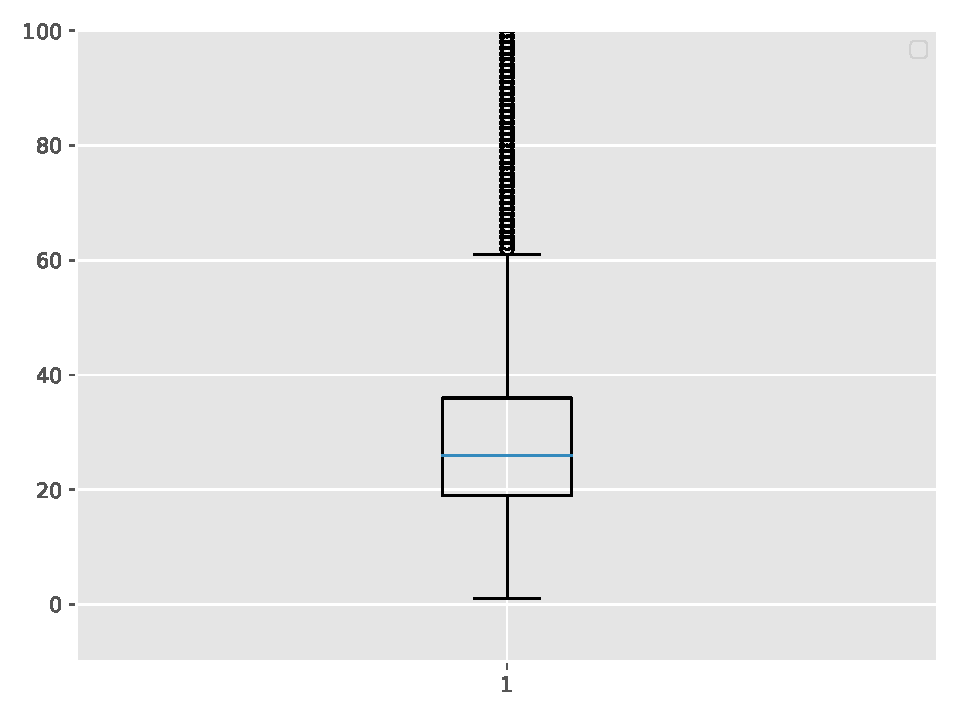
\includegraphics[width=0.75\linewidth]{images/analysis/histogram-lengths.pdf}
    \caption{Verteilung der Sequenzlängen im Datensatz }
    \label{fig:sequence-lengths}
\end{figure}

Ein Fehler in der Implementierung hat zu Beginn dazu geführt, dass für jeden Namen jeweils nur das letzte Zeichen bzw. die Stoppmarke trainiert wurde.
Interessanterweise hat selbst dieses Modell nach hinreichend langem Training zu einigen brauchbaren Ausgaben (aber hauptsächlich unlesbaren Zeichenfolgen) geführt.
Zum Vergleich mit den Ausgaben der korrekten Implementierung sind die Ausgaben des fehlerhaften Codes im Abschnitt «Resultate» (\ref{ch:results}) aufgelistet.

Bisher war das Modell so implementiert, dass jede Epoche jeweils die gleichen Trainingseinheiten erhielt.
Der Grund für dieses Vorgehen basierte auf der Annahme, dass jede Trainingseinheit mehrmals dem Modell vorgelegt werden müsse, damit der Lernprozess effektiv ist.
Diese Annahme entstand jedoch auf der fehlerhaften Implementierung, weshalb sie verworfen werden kann.

Der Nachteil war, dass das Modell eine relativ begrenztes Trainingsset zu sehen bekam.
Dieser Nachteil verstärkt sich, da durch das behobene und nun korrekt funktionierende Training noch weniger Trainingseinheiten verwendet werden.
Bei einer Median-Zeilenlänge von 26 Zeichen (siehe Abb. \ref{fig:sequence-lengths}) sowie 500 Mini-Batches à 100 Trainingsschritten werden dem Modell also:

\[ 500 \cdot \frac{100}{26} = 1'923.1 \]

gerade mal rund 1900 Zeilen der insgesamt 400'000 Zeilen gezeigt.
Damit erlernt das Modell ein sehr begrenztes Vokabular.
Die Trainingslogik soll nun so verbessert werden, dass jede Epoche einen beliebigen Ausschnitt aus allen Zeilen zum Training erhält.
Der Loader wird als Endlosgenerator implementiert.
Erreicht eine Epoche das Ende des Datensatzes, wird wieder von vorne begonnen.
Gleichwohl mit dem Datensatz, der zur Validierung herangezogen wird.
Der Generator wird also quasi als Ringspeicher implementiert wobei Trainings- und Validierungsdatensatz um die Hälfte der Länge des Gesamtdatensatzes
verschoben («Offset») ausgeliefert werden.
Damit der ganze Datensatz mindestens einmal durchlaufen wird müssten also insgesamt rund \[ 26 \cdot 422039 = 10'973'014 \] Trainingsschritte vollführt werden.
Wird von einer idealen Mini-Batch-Grösse von 100 Trainingsschritten ausgegangen, fallen insgesamt \[ \frac{109'730'14}{100} = 109'730 \] Mini-Batches an.
Damit kann die Anzahl der notwendigen Mini-Batches für einen bestimmten Prozentsatz des Gesamtdatensatzes als Funktion $ b(p, e) $ ausgedrückt werden:

\[ b(p, e) = \frac{p \cdot R \cdot S}{B \cdot e} \]

wobei $ p $ dem gewünschten Abdeckungsanteil des Datensatzes entspricht, $ e $ die Anzahl Epochen darstellt und die Konstanten $ R $, $ S $ sowie $ B $ die Anzahl Trainingssätze (Zeilen), die Median-Zeichenzahl pro Zeile sowie
die ideale Mini-Batch-Grösse repräsentieren.

Sollen also beispielsweise 25\% des gesamten Datensatzes mit 50 Epochen trainiert werden, so fallen:

\[ b(0.25, 50) = \frac{0.25 \cdot 422039 \cdot 26}{125 \cdot 50} = 438.92 \]

Mini-Batches pro an.
Diese Funktion dient dem Loader dazu, das Modell entsprechend lange zu trainieren.

\subsection{Hinzufügen eines Steuerparameters (Jahreszahl)}
\label{subsec:adding-time-component}

Jeder Trainingssatz bzw. jede Gerichtbezeichnung ist mit einem Datum versehen, an dem das Gericht zum ersten Mal
registriert wurde sowie mit einem Datum, an dem das Gericht zum letzen Mal registriert wurde.
Ein Histogram legt offen, dass die einzelnen Gerichte ungleichmässig auf die Zeit verteilt ist.
Ausserdem weist der Grossteil der Gerichte eine «Lebensdauer» von wenigen Jahren auf (siehe Abb.\ref{fig:hist-dates-datespans}).
Aufgrund letztgenannter Tatsache soll das Enddatum einfachheitshalber ignoriert werden.
Stattdessen wir das Eintrittsdatum der Eingabesequenz für das Modell angehängt.
Da nach erstem Ausprobieren das Anfügen der absoluten Jahreszahl kein gutes Training ermöglichte, wird das Jahr
als relativer Wert in einer Jahresspanne von 300 Jahren (1800 - 2100) angehängt, wobei also 0.0 dem Jahr 1800 sowie
der Wert 1.0 dem Jahr 2100 entsprechen.
Wurde zuvor das Zeichen «B» in Form eines One-Hot-Vektors $ (0.0, 0.0, 1.0, 0.0, 0.0)^{T} $ an das Modell übergeben,
so wird nun der Vektor um die Jahreszahl (z.B. 1975 = 0.583) erweitert zu $ (0.0, 0.0, 1.0, 0.0, 0.0, 0.583)^{T} $

\begin{figure}
    \centering
    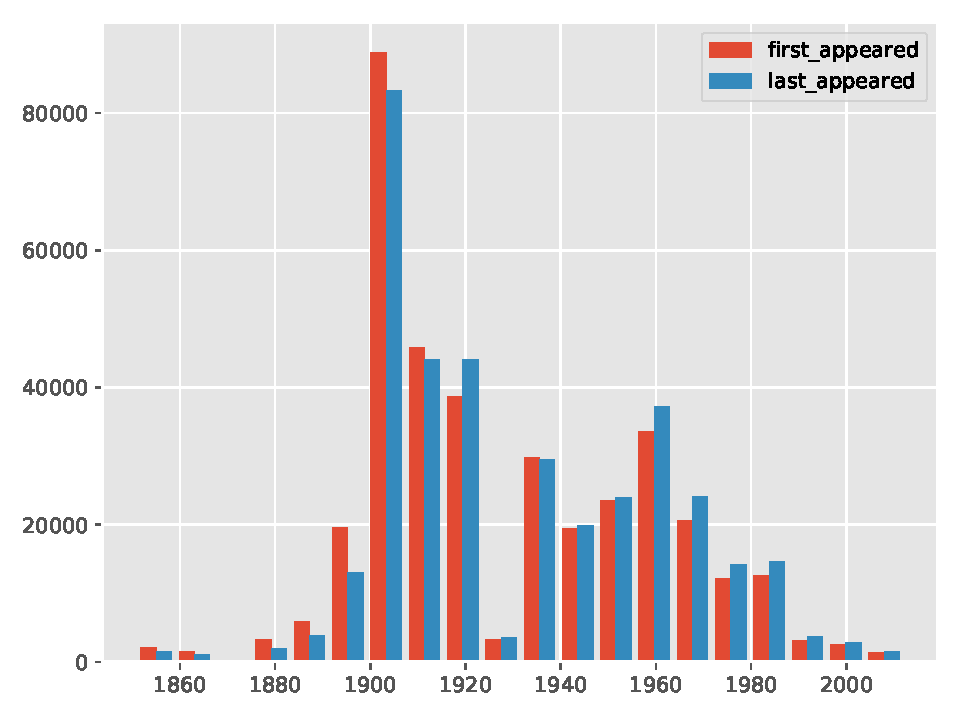
\includegraphics[width=0.75\linewidth]{images/analysis/histogram-dates.pdf}
    \caption{Zeitliche Verteilung}
    \label{fig:hist-dates-dates}
\end{figure}

\section{Erzeugung von Sequenzen}
\label{sec:model-generation}
    \chapter{Resultate}
\label{ch:results}

Dieser Abschnitt führt die durch das im vorherigen Abschnitt definierten Modell erzeugten Resultate auf und beschreibt sie.
Weil die Bewertung des Modells nur manuell und qualitativ möglich ist (d.h. Messwerte wie Präzision oder Recall korrelieren nicht zwingend
mit der wahrgenommenen Qualität der Ausgaben des Modells), ist es notwendig, dass die Ausgaben systematisch auf die verwendeten
Modellparameter zurückgeführt werden können.
Dafür wir das Modell systematisch mit unterschiedlichen Parametern trainiert, und die Resultate werden in einer
Konfigurationsmatrix aufgelistet.
Für jede Konfiguration werden die Initialsequenzen «A», «E», «I», «O», «U», «Chicken», «Steak», «Burger» und «Tomato» verwendet.
Für jede Konfiguration und jede Initialsequenz werden ausserdem jeweils drei Ausgaben erzeugt.

\begin{center}
    \begin{table}
        \centering
        \tiny
        \begin{tabular}{ |l|l|l| }

            \hline
            \textbf{} & \textbf{64 Units, val acc 49\%} & \textbf{512 Units, val acc 76\%} \\
            \hline
            \textbf{1 Layer} &
            \begin{tabular}[c]{@{}l@{}}

               Avota, Coffee, Season, Lobler, Nice Combinatiandi \\
               Ard Supremern Mambor Rolls (20 Omeley) (2 de \\
               Aspirale, Partreyning, Cocktamel, Handia Portion, Heas Ice B \\
               Eggs Holl: Coffee with Fresh Branches \\
               ERts with or Veal Holland Bour,, Butter, Salad Bowl with \\
               Extra Canfot Strawberringen Broiled Lamb Sandwich, Escelliny \\
               Isporit of Chicken \\
               Imported Sea Lemunish Limp Rib on Tarle \\
               Ice Cream, Beug \\
               Odes Potato  Rind Eocy-Fried Potatoes, Salad \\
               Oriex Coldoysh, Broth Bowl pinach) \\
               Orrerser Lobster and Butter, served with Chocolated Two Bord \\
               Undola New Chicken & Cream \\
               Utentelle Saude Craps or Peas, Coffee \\
               UVanori, Noodly Bosed with Chicken, Broiled Coffee, Rolls an \\
               Chicken and Breant \\
               Chicken Rib of Cream, Coffee Mad or Fresh Cane Yonktaa Blanch, Fre \\
               Chicken Peach Sinally Paddermi sauco \\
               Steak 25 Wenberner Dails, Beef Boiled Made Hollander with Fresh \\
               Steak cake and in with thriled smith, or Crablese, Cocktail (192 \\
               Steak, Lemon Madeluse STEAK VEGIT RYAMEL with French Fried Potat \\
               Burger with Salad and Spring Salad, sHELS SPRIMP AUL DABE \\
               Burger \\
               Burger (S.) Charent \\
               Tomato Butterrian Pie \\
               Tomato Coffee Sandwich, Pot Pork \\
               Tomato Tomato Tamered Sen Brothry Coffee, Fresh Fruits, Turlen,, \\

            \end{tabular} &
            \begin{tabular}[c]{@{}l@{}}

                Apricots, Layer Cake \\
                Arisotter's Sword Cheese, Tea and Dessert \\
                Aveck Made a OBARISION COCKTAIL (R.F.E. Regil) \\
                EWNEY COCKTAIE S9oth (Resart) \\
                Enchilada Cake \\
                English Mutton Chops, Ham, Puree Grilled in served with vinc \\
                Italian Decker \\
                Ice Cream, Parsley-Potato \\
                Italienne Lemon Horsicreme \\
                Oyster, Au Jus, French Dressing, Bread and Butter, Toast or \\
                Old English Cheese and Cream, Fresh Greens accia celery, win \\
                ORANGE Cockane \\
                Un Sirloin Steak, Dinner Stew \\
                UCYlet Bourbon Whisky \\
                Usher Cocktail \\
                Chicken Noodles, Dinner Salad \\
                Chicken Normoniscotod Beefsteak, Cookie Juice or Red Wine, Served \\
                Chicken a la Therking \\
                Steak, au Gratin Potatoes \\
                Steak a la Newburg \\
                Steak, French Fried Potatoes \\
                Burger Topps, Brandy, Fresh Mushrooms or Skresser, Cheddar Peau a \\
                Burger Scallops, Fried) \\
                Burgerstone-Crabmeat \\
                Tomato, Salad Bowl, Rolls, Coffee, Tea or Milk \\
                Tomato, Toast or Rolls, Beverage \\
                Tomato Surprise with Slices of Lettuce, Cole \\

            \end{tabular} \\
            \hline
            \textbf{5 Layers} & KZZkfvyyQexqTel & a bey \\
            \hline
        \end{tabular}
        \caption{Caption}
        \label{tab:first-sequences}
    \end{table}
\end{center}


\begin{center}
    \begin{table}
        \centering
        \begin{tabular}{ |l|l|l| }

            \hline
            \textbf{n} & \textbf{Initialsequenz} & \textbf{Generierte Sequenz} \\
            \hline
            1 & GVoRUcZybxnbknW & in Aones \\
            2 & KZZkfvyyQexqTel & a bey \\
            3 & oXvGKETlJftZHnE & SPhKAQahbgOCmjA \& pg. \\
            4 & TKWLvaUtsiBvjPm & Artonast wit Creme \\
            5 & fewKeuFYJecyCAk & Autt, cu paAte Sauce \\
            6 & ItekMqsKSONjbZj & gngn \\
            7 & KXntyJsfzrZFAJT & eatong \\
            8 & wudYekDhHOnsuPM & t \\
            9 & rOVMbLyCBbyCCSv & uAf \\
            10 & sGrYAEQfnkKxpOM & eiihg \\
            11 & jTNkWHsSswfEqhE & ing woth Mustorer) \\
            12 & bSTqiMSCZxVffMo & pshne Homatse \\
            13 & ktJyYYRuSUIJrCk & ung, D AyAnena aute,ors \\
            14 & kfoHrzlsoUGsAkY & Ah DricrTela oedt \\
            15 & DLVzoGsxmAwZgNZ & PoRrer \\
            16 & LCgtubworFrYewb & anco Hadorige \\
            17 & XchjpBUGSMyTMDq & ung \\
            19 & uNjcueOEZadlCMi & ihon w anilh Potatoast \\
            20 & UqStcroEvEehEyo & ng aust (torofffeds \\
            22 & ITiVXrEVDZXmROr & i, Are \& OoTatots \\
            23 & qweSAvVKPXrITCg & eagO \\
            26 & HfhoDhwJzEQaENT & \& Bance \\
            27 & XESvYRSRqVSVNQy & iAe, D' Arerel \& Sauce Potator \\
            28 & CswghmMaYkvPCbR & ete wite withe Bacons onito \\
            29 & tfRfupMQNvfAiaM & n Ar) \\
            30 & DdeFQkxYiMRYZdS & eupe \\
            31 & EcWjyUUvFZlzIVr & ieegs \\
            32 & seJxLpTqfwVrXap & jUTKKjCUByrALrS \& , Pon oof CTEes \\
            33 & jkAdzFdrlJDiQrI & ig anu Fueneons \\
            34 & ZItmxxUhqrlSXOI & b \\
            36 & ZhkCmYpZooVaFbs & e \\
            37 & jKbYNXXLpnbCgOd & Ait \\
            38 & wdaAgOuxYYhomCF & ith shune \\
            \hline
        \end{tabular}
        \caption{Caption}
        \label{tab:first-sequences}
    \end{table}
\end{center}

\begin{center}
    \begin{table}
        \centering
        \begin{tabular}{ |l|l|l| }

            \hline
            \textbf{n} & \textbf{Initialsequenz} & \textbf{Generierte Sequenz} \\
            \hline
            1 &  heyvAgaJnFEykXR & ROyooA SFac,a BaNooe \\
            2 &  qApRVwGkLZaRTpY & YoClNE AN COuuvE SARS \\
            3 &  hSSBSghZgvntYKW & WNOy \\
            4 &  FDtdLiovThWAABB & BaAsSA SALL IET CONDE, BRER AMBRA SUER, SIUTALIRA SLUERE BEE \\
            5 &  exvduWkBRXPNgNc & casOy BSTTESSaSTAS, Ay STENLLOWSFe \\
            6 &  pjJugwZkcVtIaHT & TEE AAa OpBu'E LAUj \\
            7 &  vYDTlKoBjHctHLM & Mer Em \\
            8 &  EATxlnekKSyyhXi & if Spakess \\
            9 &  VacBJsKUBwxBydg & gnodPHasdLirsh\& Salcok \\
            10 & DzEnFccEnDbgdHI & IEs \\
            11 & WVaBhFZTILSnQUj & jeTEEE \\
            12 & tuTluUGOpjxkryK & KraANdd Nedd \\
            13 & OKRABqePBWpocxI & Indeas \\
            14 & VzXKNFSsVfYfzlg & ge ois Ned M'llet \\
            15 & SuxVLdnvkkCacoq & qu \\
            16 & leIMviMndJaIjSb & bo org, BL OUG \\
            17 & LOFFoVRpWHMonHv & vA, TETLa \\
            19 & UkjuVIJtjoUpLIB & BTONCEETS \\
            20 & yWMmVISehLIBXoh & h \\
            22 & QHzgFhRXrsfwHnD & DhoAs,ucheredaldesri \\
            23 & sMhAWWJdrTjcjsN & Ned \\
            26 & GNGyQTKJgvxfPtK & KasagB \\
            27 & QPVDHuCtxfHrReF & F Su Sak OIp,, Ay oes Oes \\
            28 & czXXfUdrbYuxQaw & was \\
            29 & WigGaQAfkvSgyAV & Ve, LOIroua Aw CerE's \\
            30 & TfgDYRHCSXRnjDv & vELLEILLINTITEK,IS, ROUDOUYA \\
            31 & vwrTcebqyXvKChl & ls, crowmerrbous e \\
            32 & WpjVUIxzQbHbRoJ & J TEUE \\
            33 & bjXkBNwONnuriUT & TEF YEE \\
            34 & SUwXNVDHGuyrPXZ & ZANE,II  O N Ay CREp \\

            \hline
        \end{tabular}
        \caption{Caption}
        \label{tab:first-sequences-after-fix}
    \end{table}
\end{center}


\begin{center}
    \begin{table}
        \centering
        \resizebox{\textwidth}{!}{
        \begin{tabular}{ |l|l|l|l|l| }

            \hline
            \textbf{n} & \textbf{Initialsequenz} & \textbf{Generierte Sequenz 64} & \textbf{Generierte Sequenz 256} & \textbf{Generierte Sequenz 512} \\
            \hline
            1 & GVoRUcZybxnbknW & Whea & WUag Dalen & WhipTer ba ch pind Camb eits \\
            2 & TKWLvaUtsiBvjPm & moshrin  Musr rumst wchet & me & mon tarte\\
            3 & fewKeuFYJecyCAk & kfand & kglanY acol & knssaraw andderes \\
            4 & KXntyJsfzrZFAJT & T & T muthe & Te \\
            5 & jTNkWHsSswfEqhE & E, CoN Oy Lp My DfOTBRENOa  F TOINO & Eg S \& CE BLUUCR\& OTREAS, SAUL Yo Sauc & Et \& E sansere, Soulles \\
            6 & uNjcueOEZadlCMi & i, Aal are & in, & ingere \\
            7 & XESvYRSRqVSVNQy & yE, DAy NANG Lea DO CEg OAE & yUN Ef BUN SAMCE & yETT MAATEEAl \\
            8 & EcWjyUUvFZlzIVr & rF FAy Busdee B YoNNed Friodd & r ongKice & riss wAth cre \\
            9 & A & Apples & Apples & Apples \\
            10 & B & Baked apples with cream & Baked apples with cream & Baked apples with cream \\
            11 & C & Chicken broth & Chicken broth & Chicken broth \\
            12 & Chicken & n broth & n broth & n broth \\
            \hline
        \end{tabular}
        }
        \caption{Fixierte Initialsequenzen zur Untersuchung verschiedener Modellkonfigurationen}
        \label{tab:fixed-initial-sequences1}
    \end{table}

\end{center}

\begin{center}
    \begin{table}
        \centering
        \resizebox{\textwidth}{!}{
        \begin{tabular}{ |l|l|l|l|l| }

            \hline
            \textbf{n} & \textbf{Initialsequenz} & \textbf{Generierte Sequenz 64, L1, D0.1} & \textbf{Generierte Sequenz 62, L3, D0.1} & \textbf{Generierte Sequenz 64, L5 D0.1} \\
            \hline
            1 & GVoRUcZybxnbknW & in Aones & WSrh' chhompagntsos tret & Whreast \\
            2 & TKWLvaUtsiBvjPm & Artonast wit Creme & mERNT Dooo D GEN, M.lerr LNNe, Po.us PTENBe Nock FuNer rifd & mels \\
            3 & fewKeuFYJecyCAk & Autt, cu paAte Sauce & kripl & ky Snonle \\
            4 & KXntyJsfzrZFAJT & eatong & Toratt & Tinse \\
            5 & jTNkWHsSswfEqhE & ing woth Mustorer) & Es & Erg \\
            6 & uNjcueOEZadlCMi & ihon w anilh Potatoast & ih & inds \\
            7 & XESvYRSRqVSVNQy & iAe, D' Arerel \& Sauce Potator & y BRoNffrotd & yK \\
            8 & EcWjyUUvFZlzIVr & ieegs & r \& OfxTEe s & rer \\
            9 & A & kee & Apples & Apples \\
            10 & B & amb & Boiled onions, cream sauce & Baked apples with cream \\
            11 & C & \&. & \& Chicken broth & Chicken broth \\
            12 & Chicken & & n broth & n broth \\
            \hline
        \end{tabular}
        }
        \caption{Fixierte Initialsequenzen zur Untersuchung verschiedener Modellkonfigurationen}
        \label{tab:fixed-initial-sequences2}
    \end{table}

\end{center}

\begin{center}
    \begin{table}
        \centering
        \resizebox{\textwidth}{!}{
        \begin{tabular}{ |l|l|l|l|l| }

            \hline
            \textbf{n} & \textbf{Initialsequenz} & \textbf{Generierte Sequenz 64, 5000} & \textbf{Generierte Sequenz 64, 50000} & \textbf{Generierte Sequenz 64, 500000} \\
            \hline
            1 & GVoRUcZybxnbknW & in Aones & anteG in Cream & Whished Sureere \\
            2 & TKWLvaUtsiBvjPm & Artonast wit Creme & e with Milk with Bacon with Milk with Bacon with Milk with & mo\\
            3 & fewKeuFYJecyCAk & Autt, cu paAte Sauce & es) & ke \\
            4 & KXntyJsfzrZFAJT & eatong & ss & TZN CUSCACOUP PIT OY ALET Brackleass) 1/2 pot \\
            5 & jTNkWHsSswfEqhE & ing woth Mustorer) & vil)-aux champagonago & E. \\
            6 & uNjcueOEZadlCMi & ihon w anilh Potatoast & le Style & itte \\
            7 & XESvYRSRqVSVNQy & iAe, D' Arerel \& Sauce Potator & en Pee Sleate & yON \\
            8 & EcWjyUUvFZlzIVr & ieegs & eatlaine & avery & r \\
            9 & A & kee & \& & Assorted Cakes \\
            10 & B & amb & oxe & Broiled Spring Chicken Saute au gratin \\
            11 & C & \&. & rams & Cold Cocktails \\
            12 & Chicken & & & n Croquettes, Cream sauce \\
            \hline
        \end{tabular}
        }
        \caption{Fixierte Initialsequenzen zur Untersuchung verschiedener Modellkonfigurationen}
        \label{tab:fixed-initial-sequences}
    \end{table}

\end{center}

\begin{center}
    \begin{table}
        \centering
        \resizebox{\textwidth}{!}{
        \begin{tabular}{ |l|l|l|l|l| }

            \hline
            \textbf{n} & \textbf{Initialsequenz} & \textbf{Generierte Sequenz 64, 5000} & \textbf{Generierte Sequenz 256, 50000} & \textbf{Generierte Sequenz 64, 500000} \\
            \hline
            1 & GVoRUcZybxnbknW & in Aones & Wey & Whished Sureere \\
            2 & TKWLvaUtsiBvjPm & Artonast wit Creme & min & mo\\
            3 & fewKeuFYJecyCAk & Autt, cu paAte Sauce & ken Black, or Cotz, Gin & ke \\
            4 & KXntyJsfzrZFAJT & eatong & Tram Punch & TZN CUSCACOUP PIT OY ALET Brackleass) 1/2 pot \\
            5 & jTNkWHsSswfEqhE & ing woth Mustorer) & Ex& E. \\
            6 & uNjcueOEZadlCMi & ihon w anilh Potatoast & irontan, Pine Sauce & itte \\
            7 & XESvYRSRqVSVNQy & iAe, D' Arerel \& Sauce Potator & y & yON \\
            8 & EcWjyUUvFZlzIVr & ieegs & eatlaine & rI & r \\
            9 & A & kee & Anchovies & Assorted Cakes \\
            10 & B & amb & Bluefish & Broiled Spring Chicken Saute au gratin \\
            11 & C & \&. & Calf's head, fried with tomato sauce & Cold Cocktails \\
            12 & Chicken & & n croquette, with peas & n Croquettes, Cream sauce \\
            \hline
        \end{tabular}
        }
        \caption{Fixierte Initialsequenzen zur Untersuchung verschiedener Modellkonfigurationen}
        \label{tab:fixed-initial-sequences}
    \end{table}

\end{center}


\begin{figure}
    \centering
    \includegraphics[width=0.75\linewidth]{}
    \caption{Fehler in der Logik: Statt der gesamten Abfolge wird jeweils nur der letzte Buchstabe trainiert.}
    \label{fig:logic-error}
\end{figure}

512
47s 9ms/step - loss: 0.0272 - accuracy: 0.9799 - val_loss: 4.9989 - val_accuracy: 0.3500

50000
Epoch 00001: val_accuracy improved from -inf to 0.45450, saving model to checkpoints/checkpoint_100_500_50_64_1_0_15.best_val_acc.hdf5


Weiterentwicklung:

System, wo Benutzer Vorschläge bewerten kann -> Einspeisung in netz
    \chapter{Auswertung \& Ausblick}
\label{ch:analysis}

\subsection{Erhöhung der LSTM-Einheiten}
\label{subsec:increase-lstm}

\subsection{Erhöhung der LSTM-Schichten}
\label{subsec:increase-lstm-layers}

\subsection{Erhöhung der Trainingsdatensätze}
\label{subsec:increase-num-dataset}

\subsection{Erhöhen der Zufälligkeit}
\label{subsec:increase-randomness}

So wie in \autocite{dabbura} soll der nächste Buchstabe zufällig ausgewählt werden
https://docs.scipy.org/doc/numpy/reference/generated/numpy.random.choice.html

    \chapter{Fazit \& Ausblick}
\label{ch:conclusions}
    \chapter{Anhang}
\label{ch:appendix}

\begin{center}
    \begin{table}
        \centering
        \tiny
        \begin{tabularx}{\textwidth}{|>{\hsize=.1\hsize}X|>{\hsize=.45\hsize}X|>{\hsize=.45\hsize}X|}

            \hline
            \textbf{} & \textbf{64 Units} & \textbf{512 Units} \\\hline

            \textbf{1 Layer}

            &

            Art. Lugon with Lemon Steak with Santwichs, Fresh Porta \sn
            Aurabor Special \sn
            Burger Matternode, Beens \sn
            Burgerma Herring Hamburner, Jumbo Bitter \sn
            Chicken Bordeia Butterkuhe Sainds, Barolian Juice, Tortare de Long French Friedens, While Cheese \sn
            Chicken Potage sautess \sn
            Ea Roaded Mulne \sn
            Eggs of Kits Special Potato, Peas and Boiled Bollt, Dressiny \sn
            Imporied Hom Soup Cnock a la gridleys, Cabined Salad \sn
            Italian Sandwich or Onion, Mashed, Doicuols \sn
            Oce Potatoes, Fruits, Syrup, (oriles au buigs, Endoll Beef and Half-Dessert, Bacon,, Salad \sn
            OPELL CHOPPED PODS, GURLAIENURL JULIEN, ESOISTERY STEAK - PURTRROP \sn
            Ule Chambernerse Bacon, Cream of Fresh Vegetables, Couffalian Compons \sn
            U'2 Kern Inille Julien, Seddons, Coffee, Newburg, Green, grean on Whisparl \sn
            Steak Caul M. Capon \sn
            Steak with Breast, Green Pommatee with Coin cream, Mayonnaise, 1916 Jub Pers \sn
            Tomato Green Nown Lobster, Potatoes, Littlender Rois Ptupe, reef, served with De Cortored Potatoes \sn
            Tomato Slices Brandy \sn
            \sn\sn
            \textbf{Training} \sn
            Wörter: 6885, Lesbare Wörter: 69.68\%, ø-Wortlänge: 5.66\newline
            Multi: 45.7\% G: 0.52\%, E: 52\%, F: 0.46\%, I: 0.2\%, Es: 0.31\%, Dt: 0.7\% \newline
            ø-Namenslänge: 44.7, Originalität: 97.39\% \newline
            Repetition: 1.1\%, Inline-Repetition: 1.3\% \newline
            Max Val Acc: 60\%, Min Val Loss: 1.3748 \newline

            &

            All Brandy and beverages \sn
            Asparagus, Rum \sn
            Burger Holland Kbrod \sn
            Burgerbranting \sn
            Chicken Fircies with Sweetbread, Cereal Dressing \sn
            Chicken Livers Bents Harsmell \sn
            Eggs with Crisp Bacon, Fried \sn
            Eugeny Essence or Denays \sn
            I8 dienne \sn
            Imported Sardine, Bread and Butter, Pepper \sn
            O.B. Victor's White \sn
            Old Fashioned Corn \sn
            Steak Saute Mullerin \sn
            Steak Tomato Florida \sn
            Tomato au Gratin Potatoes, French fried oribroll, mornay and cereal, in meat Dill Pickle (8 years) \sn
            Tomatoes, Apple, French Fried Potatoes \sn
            Ul Soup, Iceding Cream with Toast, Rolls, With * \sn
            Ungarisnister, Tartar Sauce, Potatoes \sn
            \sn\sn
            \textbf{Training} \newline
            Wörter: 6383, Lesbare Wörter: 85.8\%, ø-Wortlänge: 5.62\newline
            Multi: 46\%, G: 0.31\%, E: 52\%, F: 0.46\%, I: 0.036\%, Es: 0.07\%, Dt: 027\% \newline
            ø-Namenslänge: 41.1, Originalität: 92.8\% \newline
            Repetition: 1.1\%, Inline-Repetition: 1.2\% \newline
            Max Val Acc: 76\%, Min Val Loss: 1.3584 \newline

            \\\hline

            \textbf{3 Layers}\newline Dropout: 5\%

            &

            Assorted Fruit Sainagido (5) \sn
            Avepilet Ory Per of Melinas \sn
            Burger Blon 2 Steak, Baked Consonfor au crabmeat, Trout - Bowl, Fried Friets of Bruefle, Fruits, Swiss Korsiurast - Lettuce Dessert and Toast and French Fried Potatoes, Coffee \sn
            Burger's in Home Clams \sn
            Chicken Chef's Bocon or Bordeal one Wine Coffee, tea or Toast or Bowl Ost. Pirener, Coinn Bon, Mimagion, Cherrions (huwey) \sn
            Chicken, Loraise Sliced Toast \sn
            Eggs with Spiped Tartar \sn
            Eio-Bread of Le roiled Coffee, Boked Corn \sn
            IGRELOSTED FRESH CALNON VANHRUNT OF TONDTER MASPY SPECED MUBERLEAGS) MICHREE \sn
            Imported and Vilrath Vegetables, Beans, Pigab Perrilles, Ling Marnicadi and with Spring Coffee, Toast, Strip, Casserole with Poples, Browned French Potatoes and Tondwed \sn
            Obsro Noudonne Choice \sn
            Oysters with Butter, Tea \sn
            Steak Saddles, Chicken Saute Person \sn
            Steak with Celery, Salad \sn
            Tomato \sn
            Tomato Steak with Fried Potatoes \sn
            U-Broiled Coffee, Vrewse or Herring, Birdo-crumb with Pork Dany Tenderloin \sn
            Urad) Ice Cereal rockfish Roast Meat salad, Bread, Pork Filet of Lincer  2) Curnet Club, Meat - Clinet Choomille \sn
            \sn\sn
            \textbf{Training} \newline
            Wörter: 10094, Lesbare Wörter: 73.6\%, ø-Wortlänge: 5.67\newline
            Multi: 44.5\%, G: 0.48\%, E: 53.95\%, F: 0.40\%, I: 0.05\%, Es: 0.13\%, Dt: 0.47\% \newline
            ø-Namenslänge: 65.8, Originalität: 98.6\% \newline
            Repetition: 0.19\%, Inline-Repetition: 2.4\% \newline
            Max Val Acc: 59.7\%, Min Val Loss: 1.3584 \newline

            &

            Asparagus ( Carrots), Cup, Shrimps, Fresh String Beans, Hollandaise \sn
            ASSORTED BREADS with Salad Bowl, Breast of Beef with Canadian Bacon, Toast or Rolls, Water Cress \sn
            Burger Hawdinne Piespund Corn with Cream Orleans \sn
            Burger Wine \sn
            Chicken a la Mornay, Mixed Green Peas and Sgr. J Loaf Cabar or Corned Beef, Baked Idaho Potato \sn
            Chicken consomme \sn
            Elberts Sherry, Barsac, Nip \sn
            English Mutton chops, smithfield, potatoes, Lettuce and Tomatoes (Gin, Waldorf Salad \sn
            India Renale, Cordials \sn
            Indle with Russian Dressing, Persimines \sn
            Order Salad Hollandaise Sauce \sn
            Our Raw Sausage, French Fried Potatoes \sn
            Steak \sn
            Steak Dinner, White Cabbage \sn
            Tomato En Casserole, Fruits or Milk \sn
            Tomato Liqueur, Bread \sn
            UND NECT CRABMEAT on Toast, French fried potato, special d'Anchovy in Toast \sn
            UR BACON, Fresh Green Peas, Baked Potato \sn
            \sn\sn
            \textbf{Training} \newline
            Wörter: 6848, Lesbare Wörter: 88.84\%, ø-Wortlänge: 5.57\newline
            Multi: 46.94\%, G: 0.13\%, E: 52.3\%, F: 0.34\%, I: 0.05\%, Es: 0.13\%, Dt: 0.1\% \newline
            ø-Namenslänge: 43.8, Originalität: 92.8\% \newline
            Repetition: 1\%, Inline-Repetition: 1.4\% \newline
            Max Val Acc: 72.12\%, Min Val Loss: 0.9165 \newline

            \\\hline
        \end{tabularx}
        \caption{Resultate verschiedener Modellkonfigurationen (Schichten vs. Units)}
        \label{tab:results-of-various-configurations-layers-units}
    \end{table}
\end{center}

\begin{center}
    \begin{table}
        \centering
        \tiny
        \begin{tabularx}{\textwidth}{|>{\hsize=.1\hsize}X|>{\hsize=.45\hsize}X|>{\hsize=.45\hsize}X|}

            \hline
            \textbf{} & \textbf{64 Units, 3 Layers} & \textbf{512 Units, 3 Layers} \\\hline

            \textbf{15\% Dropout}

            &

                Amecia Cottakages Salad, Rolls or Boiled Eggs with Rice or Y. Coffee, Potatoes \sn
                Ei Pudding, Coffee, Toast with Vegetable and Rolls, New Potatoes, Caramor't, Fresh mich and butter, bouliana Extra, \sn
                Isled C. Mixed Chicken Potatoes \sn
                Odder Cole Salad with Cocktail Steak with Broiled Potatoes \sn
                Undrot (or rumps de Potato \sn
                Chicken Roast Ham \sn
                Steak or Lettuce or Doie Parbamian. \sn
                Burger's Marinated Seavoned Fruits, Broth, Freer Soles \sn
                Tomato Chilled Oyster or Two Malurite (choice of) cream, cream Sauce \sn
                Ale Surbots Fine Potatoes, Spring Fried Vor Sweets, Metine, Fresh Fresh Fried Tea, Toast art Special Sandwich, Spring Parial Relish \sn
                EGGNED CROZBEL ORD BEEF LOWE with Potato Potatoes, Torsod on Toast or Milk \sn
                Individuale Coffee \sn
                Orange Grilled Orenge Salmon \sn
                Uldseflee with Bellou \sn
                Chicken, Stemite or Misklers Fried Vegetables with Cole Slaw and Canadien, Milk Vegetables Pineapple ALport Lemon or Spinach, Salad \sn
                Steakfy Steak, Fruits with Bongfreet \sn
                Burgerens Broth (1926, Fried or Bezeraise "Marjicot Sherry and Cole's \sn
                Tomatoes and Liqlues \sn
                \sn\sn
                \textbf{Training} \sn
                Wörter: 8887, Lesbare Wörter: 79.25\%, ø-Wortlänge: 5.55\newline
                Multi: 44.79\%, G: 0.24\%, E: 53.88\%, F: 0.37\%, I: 0.2\%, Es: 0.1\%, Dt: 0.4\% \newline
                ø-Namenslänge: 56.82, Originalität: 97.11\% \newline
                Repetition: 0.19\%, Inline-Repetition: 2.6\% \newline
                Max Val Acc: 61.3\%, Min Val Loss: 1.2872 \newline

            &

                Astor Glass and Currant Jelly (6), Coffee \sn
                Etratenrettich, natural \sn
                Imported Medium Coffee, Tea or Milk \sn
                Onton Boukinger, 1863, Julian Bloxfervers, Apple Sauce, Viennoise Dressing, Potatoes, Lettuce, Toast, Cream \sn
                Unleyskating in Crackers \sn
                Chicken Noodles, Toast, Coffee, Tea or Milk \sn
                Steak Sandwich - Sliced Apple Pastry \sn
                Burger Bordeaux \sn
                Tomato a la Saffron Drink \sn
                Ala Carves Filets of Salmon and Butter, Sauce Royal (43 Years) \sn
                Enstew Corn fritters, garnished with Dinner Sweet, Saute Omeritaine, Fresh Green Peas, Cheese Sandwich \sn
                Imported Toast, Hard Boiled Egg, Fresh Greens with Florida Salts of Crabmeat a la Nopoleun (Bordeaux, Mock Waffle) \sn
                Old Taxmerowliel Medos, Curacao Potatoes \sn
                Under Small Chicken with Broiled or Fried, Queen \sn
                Chicken And Whipped Potatoes, Bread, Butter, Beverage \sn
                Steak Sandwich \sn
                Burgers French or Carafelle and wine, mixed vegetables saute with baked potatoes \sn
                Tomato Gritzers \sn
                \sn\sn
                \textbf{Training} \sn
                Wörter: 6847, Lesbare Wörter: 89.0\%, ø-Wortlänge: 5.71\newline
                Multi: 45.27\%, G: 0.19\%, E: 53.95\%, F: 0.4\%, I: 0.0\%, Es: 0.01\%, Dt: 0.14\% \newline
                ø-Namenslänge: 44.85, Originalität: 94.88\% \newline
                Repetition: 1.0\%, Inline-Repetition: 1.2\% \newline
                Max Val Acc: 75.85\%, Min Val Loss: 0.7852 \newline

            \\\hline
            \textbf{60\% Dropout}

            &

                Andilly Blals Cheders, Marmapily, Jol Tupeloiled milk \sn
                Engruse Rot \sn
                Imported CreamnPotatoes, PLIKED LEIMTED (Hegs) of Potatoes \sn
                O. Chicken Milk Saupe \sn
                Ucarina Salad with Broilnd Torron, salmw Egg - Yeger Hegerroma Souse with Keaf Swicilo, Jingheous Prope, Red Pouled a la Foller bais \sn
                Chicken or Persker, teas Salad, Tatielatin Salad, Stew, Eggs, Creamed Beef, or Jambrad Salad \sn
                Steaked Trouy Oxsteel Bishlon Toasts \sn
                Burger deflalt of Sprind Vermout, Derbonled Potato Coffee \sn
                Tomato Seapool, Mevos Saldw Rice Sauce \sn
                Alle Parmelor Smicche ol Peas, Fillet Crenmed French Fresh De Toast, Blailed Potatoes, Berny or Rooll, ores, Choited Steaked Gwull Iseled Per on Blanger Steam and Bottles, Lill, Greens webth Chicken Wester Ice Rotch \sn
                Emelesolbalme Cakfort (Ici \sn
                Imeliente Roy Cottole, Buttern Ore \sn
                Opbeer Cread a la scrimt Ice Fot \sn
                UcE THalled Vibflel \sn
                Chicken Broiled Egg Stnak, Champagne and Bowls, Farsai Bared, Jelly and french Cream; Totatoes of Imerwits and Tinnarisite \sn
                Steak Bricken, Solv Clea Parshing Swueted Fremh Fried and Teas, Orinach \sn
                Burgerelleds Sin Spring Harn Coffee \sn
                Tomatoes Whanz din \sn
                \sn\sn
                \textbf{Training} \sn
                Wörter: 8090, Lesbare Wörter: 59.18\%, ø-Wortlänge: 5.68\newline
                Multi: 41.24\%, G: 0.79\%, E: 54.97\%, F: 0.73\%, I: 0.41\%, Es: 0.27\%, Dt: 1.56\% \newline
                ø-Namenslänge: 52.76, Originalität: 97.9\% \newline
                Repetition: 0.5\%, Inline-Repetition: 1.3\% \newline
                Max Val Acc: 52\%, Min Val Loss: 1.6069, Early Stopping \newline

                &

                American Blin, Quene Spices, Fried Chicken, Corn Fritter  Special (Fresh Tenderloin of Olives Cocktail \sn
                Escalloped Pineapples and fresh Asparagus tips of veal with rice style \sn
                Imported Blue Sherbet \sn
                Our lima Beans \sn
                U. Groven Bellevo Tomato Jamaica Ham and Casen's \sn
                Chicken, CornndBeer, Mushrooms, Baked Rice, Oysters, Choice of Cocrail Cocktail \sn
                Steak, Red Spinach \sn
                Burger mirns 1 Fried Filet \sn
                Tomato Supreme Fr Sterring \sn
                American Cheese, Toast or Rolls, Coffee, Tea or Milk \sn
                Eggs and Italian Bacon, Broiled, Fresh, Vegetables, Sour Cream, Indian Rye, Broiled potatoes, beefsteak, potatoes, broiled macaroon \sn
                Irish Fruits en Brochette, Cocktail \sn
                OLD ENGLISH TOMATO \sn
                Uper Clams \sn
                Chicken Livers, Toast or Rolls, Sweet Potatoes \sn
                Steak Omelette, Blackbraenberry Scotia Supreme with Hot Saldage \sn
                Burger Boneless \sn
                Tomato toast stew \sn
                \sn\sn
                \textbf{Training} \newline
                Wörter: 7390, Lesbare Wörter: 90.35\%, ø-Wortlänge: 5.65\newline
                Multi: 45.9\%, G: 0.11\%, E: 53.39\%, F: 0.31\%, I: 0.08\%, Es: 0.05\%, Dt: 0.11\% \newline
                ø-Namenslänge: 48.06, Originalität: 94.24\% \newline
                Repetition: 1.7\%, Inline-Repetition: 1.9\% \newline
                Max Val Acc: 72.3\%, Min Val Loss: 0.8983 \newline
            \\\hline
        \end{tabularx}
        \caption{Resultate verschiedener Modellkonfigurationen (Dropout)}
        \label{tab:results-of-various-configurations-dropout}
    \end{table}
\end{center}




\begin{center}
\begin{table}
\centering
\tiny
\begin{tabular}{ |l|l|l| }

\hline
\textbf{} & \textbf{64 Units, 1 Layer} & \textbf{512 Units, 3 Layers (Dropout 5\%)} \\
\hline
\textbf{25\%} &
\begin{tabular}[c]{@{}l@{}}
\\
Aporo Dut, with Salad \\
A8nolich a la StIIDre Sweetofres \\
Aureung Gebary au \\
Eschiol, Otelette \\
E balised of sayferne Shotare \\
Estrabse Whitts de chicodols \\
Ichidzey Flocon,, Tourss \\
Impormoin Crops \\
Ipfish with PingFlouffien \\
Oldimber Hortons, Veartig \\
Omeles, Rigemmen \& Couques \\
Oysterster Partini \\
UYerugres Immerking \\
Ufflesbines Fribston \\
Ugg Fry-chable fort \\
Chicken of tibued Suplet sompete Sauces a la Pillet \\
Chicken, Zerter Sidpaille Harbuese \\
Chicken Whitse matarien, a la Bleemes in \& CUS. \\
Steak Muderoen \\
Steak-dopatie, \\
Steak deuiel Denca patse, Clutton \\
Burger with [plees \\
Burger Beer, Bostern with Hraisel \\
Burgeres Rooss \\
Tomato botale \\
Tomato, (Whived \\
Tomatoes soumore \\
\\
\textbf{Training} \\
Wörter: 91, Lesbare Wörter: 31.9\%, \\
Originalität: 100\%
ø-Wortlänge: 6.12, ø-Namenslänge: 23.59, \\
Max Val Acc: 59.83\% (Early Stop), Min Val Loss: 1.3662\\

\end{tabular} &
\begin{tabular}[c]{@{}l@{}}
\\
Aniguillo de parme \\
Asparash Red Lorn Chocolate \\
Anguille de Barbelere servicettes, 16g \\
Erdbeer minerela \\
Essotti fennenta \\
Etten \\
Imperial of Graqu Sweet Rests \\
Italian biscuit \\
Iveli of Sparkling Johnni Fruit Salad \\
Oeufs en crocoli a-ni \\
Oeufs Fried in Butter \\
Okra Tonke \\
Unger's Spcire Ice \\
Umarocasioni \\
Uvera enforica \\
Chicken Nayonse Maruelpi \\
Chicken subraie in gratin \\
Chicken --Terrine and Yoin, Buchino Chantilly, Sauce Mayonnaise \\
Steak Persillee \\
Steak de Rougetes \\
Steak & Rie ersjeg Rhine Wine \\
Burger Holtheimer mit Zilanes, petit zako \\
Burger Salad \\
Burger Kase Boscolite \\
Tomato, st. Julien \\
Tomato \\
Tomato Tostado 1955, Innesara \\
\\
\textbf{Training} \\
Wörter: 90, Lesbare Wörter: 64.4\%, \\
Originalität: 92.59\% \\
ø-Wortlänge: 5.81, ø-Namenslänge: 22.1, \\
Max Val Acc: 60.4\%, Min Val Loss: 1.3448 \\

\end{tabular} \\
\hline
\textbf{200\%} &
\begin{tabular}[c]{@{}l@{}}
\\
Aptiple de Caunas with Finota of Cucry with Vegetables \\
AGr crooket sauce \\
A Burgono Hot Estreast of Toast, Roll with Bass, Lettuce and \\
Escreests special , and, Eison, c \\
Eschire (3) (2) Cufue \\
Eschweins \\
Imperial Cuffee with Galliero Dry, Bacon Piladed and French \\
Itali of Cold, Choister Corter \\
Indiesticangus ) Red Salmon (verndi.) with Pie \\
Old Grilled Shrimp Steam \\
Ofzflamifina. Tram, Pie \\
Oysters (Anloos \\
Undle Sautere and Scotchara \\
Ungered Finet Water \\
UB. Marger (Imperiauche) \\
Chicken Scrambled (lettle \\
Chicken Special Brown \\
Chicken Sandwich, Garratac oder Cake in Toast, peppers and for \\
Steak, Cakested or Thips \\
Steakkaring - Grands Sandwich \\
Steak, Frence L.M \\
Burger AY" Red Toit \\
Burger Beetsalad with and Lobster en Chips \\
Burger Sere Sandwich Sandwich with Cardo Price \\
Tomato Bounlion Cheese \\
Tomato Pork, Gall's French Brocc's, Spring Lamb, Cole en Beustur \\
Tomato Perling Sauce, Wum \\
\\
\textbf{Training} \\
Wörter: 131, Lesbare Wörter: 62.6\%, \\
Originalität: 100\% \\
ø-Wortlänge: 5.53, ø-Namenslänge: 31.74, \\
Max Val Acc: 59.83\% (Early Stop), Min Val Loss: 1.3662\\

\end{tabular} &
\begin{tabular}[c]{@{}l@{}}

AFTIAN PICKLE, BISCUITS \\
Apple Snapper, Creamed Onions Supreme \\
ASPARADUS FRIED CHICKEN \\
En Gecand Home Made Tropical \\
ESCORODED SNEW, Dinner Salad \\
English Mutton Chop, Counn Bread, Tomatoes \\
IN HUNGARIAN PALD DRINKSUPPE \\
Imported Swiss Cheese, Green Peas, French Fried Potatoes, Mi \\
Invly Fleischhine, Zwack \\
Omelet with Mixed Salad \\
Orange Ice Cream \\
O'Brien Oyster Stew, Sandwich, Rice Salad \\
Un Orange Juice, Nips, Plain Bacon, String Beans, Tartar Sau \\
Uven Cabbag., Bread and Butter \\
Umley's Stor Korbae Our or Royal Spreadek \\
Chicken Livers, Betty Pepper \\
Chicken Soup plate: Carrots, Toast, Beets, Toast or Rolls and Butt \\
Chicken Salad with Poached Egg \\
Steak Club \\
Steak and Tara Blend of Corn Beef, Tongue and Coffee or Rolls, C \\
Steaks en Casserole \\
Burger Louisiana Pie, Mayonnaise \\
Burger Royal Cocktail \\
Burger-Petite Maison \\
Tomato Surprise \\
Tomatoes, Extra Lima Beans, Hard Boiled Potato \\
Tomato, Cole Slaw \\
\\
\textbf{Training} \\
Wörter: 181, Lesbare Wörter: 86.7\%, \\
Originalität: 81.48\% \\
ø-Wortlänge: 5.42, ø-Namenslänge: 32.29, \\
Max Val Acc: 72.12\%, Min Val Loss: 0.9165 \\

\end{tabular} \\
\hline
\end{tabular}
\caption{Resultate verschiedener Modellkonfigurationen (25\% Datensatz vs. 200\% Datensatz)}
\label{tab:results-of-various-configurations}
\end{table}
\end{center}



\begin{center}
    \begin{table}
    \centering
    \tiny
    \begin{tabularx}{\textwidth}{|>{\hsize=.1\hsize}X|>{\hsize=.45\hsize}X|>{\hsize=.45\hsize}X|}

        \hline
        \textbf{} & \textbf{64 Units, 1 Layer} & \textbf{512 Units, 3 Layers (Dropout: 5\%)} \\\hline
        \textbf{1900}

        &

        A THIPPONETTEE PEICKEL on Cereal Forast Pudding, 10 83 \sn
        Alurine \sn
        Burger Rolls, French Fried Rouger \sn
        Burgery Madetage a l'Apolito \sn
        Chicken Lamb Chops, Toast with Salad, All Bake, Salmon Plate, Gintsies \sn
        Chicken Shrimp trout (with per toosted with Gray Bread, Rye Hal Brooch, Rolls Served with Devilly, French Friled Groos \sn
        Eartre Kimble on Parrosas, Green Salad, Salmon and Eggs in Broiled Baralian Ing Derole Salad \sn
        Eprwerher Shrimps Griold Tamate, Kortingny Lima Ry Le Cracaionille Sandwich White Creamed Beefed Ham or Brice, Spaghetti, Chickle Salad, Mette (6) with Cream, Cream and Onions, Bouthion Wine, Half Brundons, Pork with Blue Beef, Hail Salfe, Fresh Chilken \sn
        Imported Scotney, Seas \sn
        Itali Cerrouite \sn
        Ohe Libre Lemon Potatoes, Ponmossored Leubared Pit Rice and New Bacon Tookey \sn
        Onions of Deprishnish \sn
        Steak \sn
        Steak Cinnan Dressisper Broiled of Lobster, Crab, Newburg Lizkfrais, Clab Rice Slice, Hadfian with Buttered On Passeery Cocktail \sn
        Tomato, French Fried, Vermalais, Chicken, Cole Slaw of Per Cake \sn
        Tomatoes Herrine, Bread and Butter, Toost Bown, Saute Pork, Mears \sn
        Uld Meuniniere Pork Chow Lamb Tarlowners \sn
        Umenty Cornadol, Kollzz Coffee, Tea, Potatoes, Parsley Hambor Lettuce, Essort Saute, Brandnerise) \sn
        \sn\sn
        \textbf{Training} \sn
        Wörter: 7075, Lesbare Wörter: 68.16\%, ø-Wortlänge: 5.72\newline
        Multi: 43.72\% G: 0.45\%, E: 53.84\%, F: 0.55\%, I: 0.31\%, Es: 0.43\%, Dt: 0.66\% \newline
        ø-Namenslänge: 46.36, Originalität: 97.49\% \newline
        Repetition: 1.0\%, Inline-Repetition: 1.1\% \newline
        Max Val Acc: 60\%, Min Val Loss: 1.3748 \newline

        &

        Aiguilets of Glass Waters, Coffee, Fresh Mushrooms, New Peas, Currant Jelly \sn
        Assorted Lamb Wine Sauce Nut Soup \sn
        Burger per port Brede \sn
        Burger-Beer Oranges \sn
        Chicken Salad: Noodles or Milk \sn
        Chicken with Amontillad Salad with Sweet, Vegetable, Salad \sn
        Eden Cream, Beas, Potatoes, Cream or Rolls \sn
        Extra Vermouth Made Fruits, Cereal \sn
        Imported \& Fruits and Ham, Two Vegetables, Salad Bowl, Fresh Murway, Tartar Sauce, French Fried Potatoes \sn
        Imported Herring, Toast \sn
        Old Assorted Cold Cuts \sn
        Old Mandhousses, Salad Orange, apple Juice - Any Cocktail \sn
        Steak potatoes and served with Asparagus, Tartar \sn
        Steak, served from cocktail \sn
        Tomato or Sea Bass, Yumber Rosengat, French Fried, Grill Bread, Butter, Lemon \sn
        Tomato Stuffed with Mushrooms or Mushrooms \sn
        Uliente Riesling, Choice Sherbets \sn
        Undernitz, Grilled Tomato, Sausage, Sparkling Burgundy Sweetbreads, Horseradish, Bread and Butter \sn
        \sn\sn
        \textbf{Training} \sn
        Wörter: 7169, Lesbare Wörter: 89.24\%, ø-Wortlänge: 5.66\newline
        Multi: 45.34\% G: 0.06\%, E: 53.96\%, F: 0.23\%, I: 0.06\%, Es: 0.06\%, Dt: 0.26\% \newline
        ø-Namenslänge: 46.53, Originalität: 95.27\% \newline
        Repetition: 1.3\%, Inline-Repetition: 1.9\% \newline
        Max Val Acc: 74.7\%, Min Val Loss: 0.8239 \\\hline

        \textbf{2000}\newline Dropout: 5\%

        &

        Art. Lugon with Lemon Steak with Santwichs, Fresh Porta \sn
        Aurabor Special \sn
        Burger Matternode, Beens \sn
        Burgerma Herring Hamburner, Jumbo Bitter \sn
        Chicken Bordeia Butterkuhe Sainds, Barolian Juice, Tortare de Long French Friedens, While Cheese \sn
        Chicken Potage sautess \sn
        Ea Roaded Mulne \sn
        Eggs of Kits Special Potato, Peas and Boiled Bollt, Dressiny \sn
        Imporied Hom Soup Cnock a la gridleys, Cabined Salad \sn
        Italian Sandwich or Onion, Mashed, Doicuols \sn
        Oce Potatoes, Fruits, Syrup, (oriles au buigs, Endoll Beef and Half-Dessert, Bacon,, Salad \sn
        OPELL CHOPPED PODS, GURLAIENURL JULIEN, ESOISTERY STEAK - PURTRROP \sn
        Ule Chambernerse Bacon, Cream of Fresh Vegetables, Couffalian Compons \sn
        U'2 Kern Inille Julien, Seddons, Coffee, Newburg, Green, grean on Whisparl \sn
        Steak Caul M. Capon \sn
        Steak with Breast, Green Pommatee with Coin cream, Mayonnaise, 1916 Jub Pers \sn
        Tomato Green Nown Lobster, Potatoes, Littlender Rois Ptupe, reef, served with De Cortored Potatoes \sn
        Tomato Slices Brandy \sn
        \sn\sn
        \textbf{Training} \sn
        Wörter: 6885, Lesbare Wörter: 69.68\%, ø-Wortlänge: 5.66\newline
        Multi: 45.7\% G: 0.52\%, E: 52\%, F: 0.46\%, I: 0.2\%, Es: 0.31\%, Dt: 0.7\% \newline
        ø-Namenslänge: 44.7, Originalität: 97.39\% \newline
        Repetition: 1.1\%, Inline-Repetition: 1.3\% \newline
        Max Val Acc: 60\%, Min Val Loss: 1.3748 \newline

        &

        American Cheese Crack, Toasted Rice and Chicken \sn
        Eggs a la Bordcart a la Kuffare \sn
        Indio Hagnnoten Beer \sn
        Oysters Pineapple Cooked Potatoes \sn
        USSON OYSTERS \sn
        Chicken a la Menthe, Broiled Konnello es Holstein or Onions, Broiled Olive (2), Grilled Vegetable White Port \sn
        Steak a la Miltg \sn
        Burger Peter copper, Minute, String Beans, Mashed Potatoes, Bread with Mashed Potatoes, Sweet Potatoes, Desserte, Coffee \sn
        Tomato Turkey Maryland] \sn
        A'baris, American Sauve Cocktail \sn
        Eggs Finest 1/1 lusienne potatoes \sn
        Ice Cream on Toast or Fried Corned Coffee, Toast, Toast, Tea or Rice \sn
        Oldan Cheese, Toast or Rolls \sn
        Umprestor's Leek, Fried Onions \sn
        Chicken a l'Anglaise, Copped Potato, Cole Slaw, French Fried Potatoes, Broiled Live Lobster, Stuffed with Toast or Rolls, Newburg, Potato Salad, Glass of Asparagus \sn
        Steak Dinner: \sn
        Burger \sn
        Tomato Stuffed in Caff with Braised Spark Salad) \sn
        \sn\sn
        \textbf{Training} \sn
        Wörter: 7294, Lesbare Wörter: 89.08\%, ø-Wortlänge: 5.58\newline
        Multi: 46.5\% G: 0.21\%, E: 52.46\%, F: 0.46\%, I: 0.16\%, Es: 0.06\%, Dt: 0.12\% \newline
        ø-Namenslänge: 44.7, Originalität: 93.34\% \newline
        Repetition: 1.1\%, Inline-Repetition: 1.3\% \newline
        Max Val Acc: 72.12\%, Min Val Loss: 0.9165 \\\hline
\end{tabularx}
\caption{Resultate bei Verwendung unterschiedlicher Jahreszahlen}
\label{tab:results-of-various-years}
\end{table}
\end{center}


\begin{center}
\begin{table}
\centering
\begin{tabular}{ |l|l|l| }

\hline
\textbf{n} & \textbf{Initialsequenz} & \textbf{Generierte Sequenz} \\
\hline
1 & GVoRUcZybxnbknW & in Aones \\
2 & KZZkfvyyQexqTel & a bey \\
3 & oXvGKETlJftZHnE & SPhKAQahbgOCmjA \& pg. \\
4 & TKWLvaUtsiBvjPm & Artonast wit Creme \\
5 & fewKeuFYJecyCAk & Autt, cu paAte Sauce \\
6 & ItekMqsKSONjbZj & gngn \\
7 & KXntyJsfzrZFAJT & eatong \\
8 & wudYekDhHOnsuPM & t \\
9 & rOVMbLyCBbyCCSv & uAf \\
10 & sGrYAEQfnkKxpOM & eiihg \\
11 & jTNkWHsSswfEqhE & ing woth Mustorer) \\
12 & bSTqiMSCZxVffMo & pshne Homatse \\
13 & ktJyYYRuSUIJrCk & ung, D AyAnena aute,ors \\
14 & kfoHrzlsoUGsAkY & Ah DricrTela oedt \\
15 & DLVzoGsxmAwZgNZ & PoRrer \\
16 & LCgtubworFrYewb & anco Hadorige \\
17 & XchjpBUGSMyTMDq & ung \\
19 & uNjcueOEZadlCMi & ihon w anilh Potatoast \\
20 & UqStcroEvEehEyo & ng aust (torofffeds \\
22 & ITiVXrEVDZXmROr & i, Are \& OoTatots \\
23 & qweSAvVKPXrITCg & eagO \\
26 & HfhoDhwJzEQaENT & \& Bance \\
27 & XESvYRSRqVSVNQy & iAe, D' Arerel \& Sauce Potator \\
28 & CswghmMaYkvPCbR & ete wite withe Bacons onito \\
29 & tfRfupMQNvfAiaM & n Ar) \\
30 & DdeFQkxYiMRYZdS & eupe \\
31 & EcWjyUUvFZlzIVr & ieegs \\
32 & seJxLpTqfwVrXap & jUTKKjCUByrALrS \& , Pon oof CTEes \\
33 & jkAdzFdrlJDiQrI & ig anu Fueneons \\
34 & ZItmxxUhqrlSXOI & b \\
36 & ZhkCmYpZooVaFbs & e \\
37 & jKbYNXXLpnbCgOd & Ait \\
38 & wdaAgOuxYYhomCF & ith shune \\
\hline
\end{tabular}
\caption{Caption}
\label{tab:first-sequences}
\end{table}
\end{center}

    \chapter*{Glossar}
\addcontentsline{toc}{chapter}{Glossar}
\renewcommand{\glossarysection}[2][]{}

\printglossaries





    \printbibliography[<options for printing>]

    \listoffigures


\end{document}
